
\medskip
Afin de ne pas surcharger la figure, ici, on n'aura tracé les traits de lecture graphique que quand le sujet le demande.

\parbox[t]{0.5\linewidth}{
	\begin{enumerate}\item \begin{enumerate}
			\item On lit que 4 a un antécédent par la fonction $g$, qui est 2.	
			\item On a le tableau de valeurs suivant : 	
			\hfill~
			
\begin{tabularx}{0.95\linewidth}{|*{6}{>{\centering\arraybackslash}X|}} \hline
$x$&$-2$&0&4&6\\ \hline
$g(x)$&12&8&0&$-4$\\ \hline
\end{tabularx}\hfill~
	\end{enumerate}
		\item 
			\begin{enumerate}
				\item On a : $f(-2) = 2\times (-2) = -4$.
				\item On a : $f(3) = 2\times 3 = 6$.
				\item La fonction $f$ est linéaire, donc elle sera représentée par une droite, passant par l'origine du repère.
			
En utilisant les réponses aux deux questions précédentes, on peut dire qu'elle passera à la fois par le point A$(-2~;~-4)$ et par B$(3~;~6)$.
			
Voir l'annexe complétée ci-contre : 
			\end{enumerate}
		\item Le point d'intersection S dont l'abscisse est égale à 2.
\end{enumerate}}
\hfill 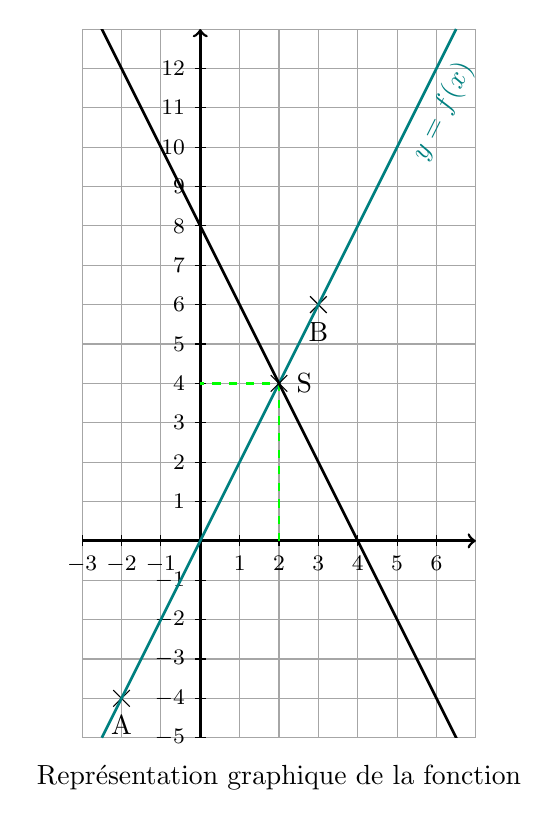
\begin{tikzpicture}[x=5mm,y=5mm,baseline={(current bounding box.north)}]
\draw [gray!70,xstep=1,ystep=1] (-3,-5) grid (7,13);
\draw[line width=1pt,->] (-3,0)--(7,0);
\draw[line width=1pt,->] (0,-5)--(0,13);
\foreach \x in {-3,-2,-1,1,2,...,6}{
	\draw (\x,2pt)--(\x,-2pt) node[below]{{\footnotesize $\x$}};}
\foreach \x in {-5,-4,...,-1,1,2,...,12}{
	\draw (2pt,\x)--(-2pt,\x) node[left]{{\footnotesize $\x$}};}
\draw[shift={(-2,-4)}] (-3pt,-3pt)--(3pt,3pt) (-3pt,3pt) -- (3pt,-3pt) (0,0) node[below=1mm]{A};
\draw[shift={(3,6)}] (-3pt,-3pt)--(3pt,3pt) (-3pt,3pt) -- (3pt,-3pt) (0,0) node[below=1mm]{B};

\draw[line width = 1pt, teal] (-2.5,-5)--(6.5,13) node[pos=0.9,sloped,below]{$y=f(x)$};
\node at(2,-6) {Représentation graphique de la fonction};
\draw[green,dashed,line width=1pt] (2,0)--(2,4)--(0,4);
\draw[shift={(2,4)}] (-3pt,-3pt)--(3pt,3pt) (-3pt,3pt) -- (3pt,-3pt) (0,0) node[right=1mm]{S};
\clip (-3,-5) rectangle (7,13);
\draw [line width=1pt] (-3,14)--(7,-6);
\end{tikzpicture}
\hfill ~

\begin{enumerate}[start=4]
	\item \begin{enumerate}
		\item Résolvons l'équation :
		
		\begin{tabbing}
			$2x = -2x + 8$\=$\iff 4x = 8$\\
			\>$\iff x= 2$
		\end{tabbing}
		
L'équation a une unique solution : 2.
		
		\item L'équation que nous venons de résoudre est : $f(x)=g(x)$, puisque l'on a $g(x) = 2x$ et $g(x)=-2x+8$ pour tout $x$.
		
La solution trouvée est donc la valeur de $x$ qui donne une même image pour la fonction $f$ et la fonction $g$, c'est donc l'abscisse du point d'intersection S des deux courbes représentatives, ce qui confirme notre lecture graphique de la question \textbf{3.}.
	\end{enumerate}
\end{enumerate}

\vspace{0,5cm}

